Our working hypothesis, as outlined in the Introduction, is that
mirror structures will enable a biological system such as a primate or
a human being to ``rehearse'' the actions it performs in a determined situation,
as this situation is evoked by seeing, hearing, smelling, etc. A useful distinction
naturally arises then between active and passive sensory modalities. An active
modality is the perception of the system's own actions through proprioception
and tactile feedback, whereas a passive modality is simply the perception
of the environment, generally through distal modalities\footnote{We denote here,
with the term \emph{distal}, sensory modalities which convey information about
events outside the system's peripersonal space.}.

We also claim that additional information given by the mirror structure greatly
helps a biological system understand its environment. In the first place,
multi-modal perception \cite{...} already gives to a biological system a much
richer and robust way of dealing with noisy/incomplete information --- as an
example, to determine whether an animal is facing a predator or a prey, as well
as in a courtship ritual. Regarding the distinction between passive and active
modalities, since active modalities are seldom available in nature, it is supposed
that mirror structures reconstruct the passive ones from the active ones, in order to
approximate the benefit of multi-modal learning.

We then assume that there exists a mapping between (sets of) patterns belonging to
active and passive modalities; for example, for a human being, it should be possible
to reconstruct to a good degree of approximation the way to grasp a mug from the
sight of a so-far unseen mug. In the framework of statistical learning, we will
then be looking for a \emph{perception-to-action map} (PAM), something like what
is shown in Figure \ref{fig::implementation}.

\begin{figure}[h!]
  \centering
  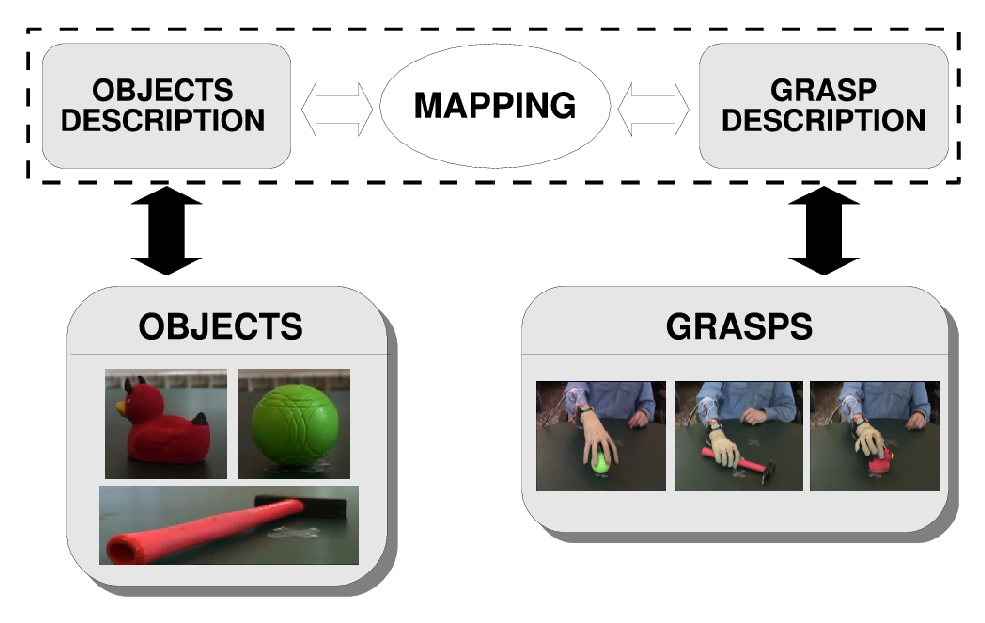
\includegraphics[width=0.7\textwidth]{images/schema_implementazione}
  \caption{An instance of the framework we propose: estimating a
   mapping between appropriate visual descriptions of objects and
   classes of grasp actions.}
  \label{fig::implementation}
\end{figure}

A PAM will be functionally akin to a mirror structure, able to tell us ``what
to do'' with ``what we perceive''. A PAM will be built by statistical learning,
probably regression, applied to a dataset of pairs (distal feature / proximal
feature) gathered, in general, from live subjects. Biologically speaking,
the equivalent of this training phase is represented by the association between
distal perception and \emph{manipulation} an animal performs when, as an infant,
plays or fights, or simply babbles around.

A paradigmatic example is that of a human infant learning how to grasp an object:
by repeatedly trying to apply, e.g., a cylindric grasp to a bottle, it will learn
not only to do it more and more efficiently, but also that a bottle is better be
grasped cylindrically when moving it or bringing it close to the mouth. Later on,
the sight of a bottle will remind the young human what one of the correct grasps
is for that particular object.

Notice that in general the PAM is trying to solve an ill-posed problem, since
naturally many possible different instances of a passive modality can correspond
to a single active one. In the above example, any human knows that both a hammer
and a bottle can be grasped cylindrically\footnote{the nomenclature of grasp types
loosely follows that of Cutkosky \cite{cutkosky}.}), and as well that a mug can be
handled either cylindrically or by the handle.

In general, at the time of deciding
what kind of grasp to use, the desired task will come into play. Let it suffice
then, by now, to state that the output of a PAM will not be, in general, a single
instance of a proximal modality, but rather a probability distribution over them.
For example, the sight of a mug will elicit, with different probabilities, the
cylindrical grasp, the pinch grip, the handle grip. This makes the problem slightly
harder, but at the same time makes the obtained system more realistic.

So, a PAM will enable us to recover a probability distribution over proximal
modalities, given a distal modality. This operation will be called \emph{proximal
priming} in the following.






%\begin{figure}[h!]
%	\centering
%	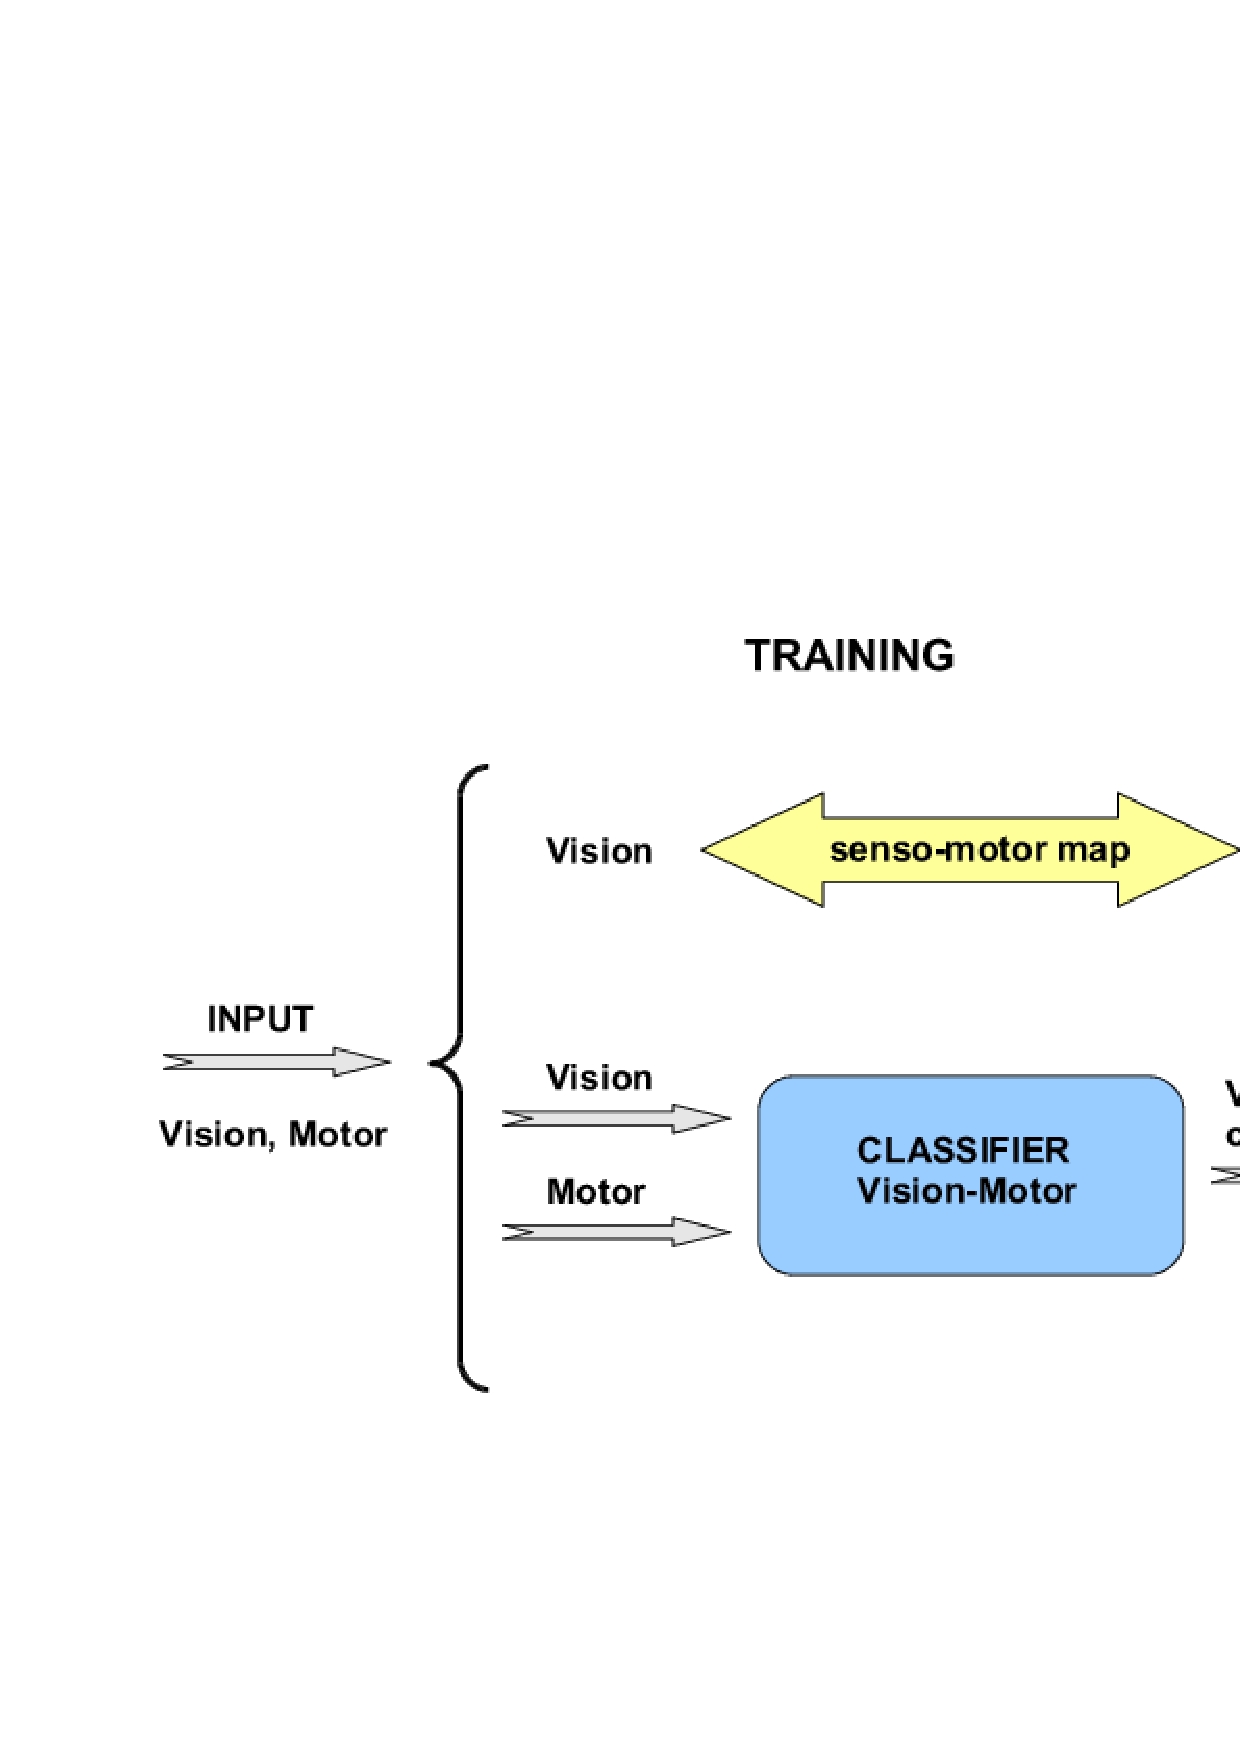
\includegraphics[width=0.7\textwidth]{images/train_fig}
%	\caption{blabla}
%	\label{fig:training-scheme}
%\end{figure}
%
%\begin{figure}[h!]
%        \centering
%        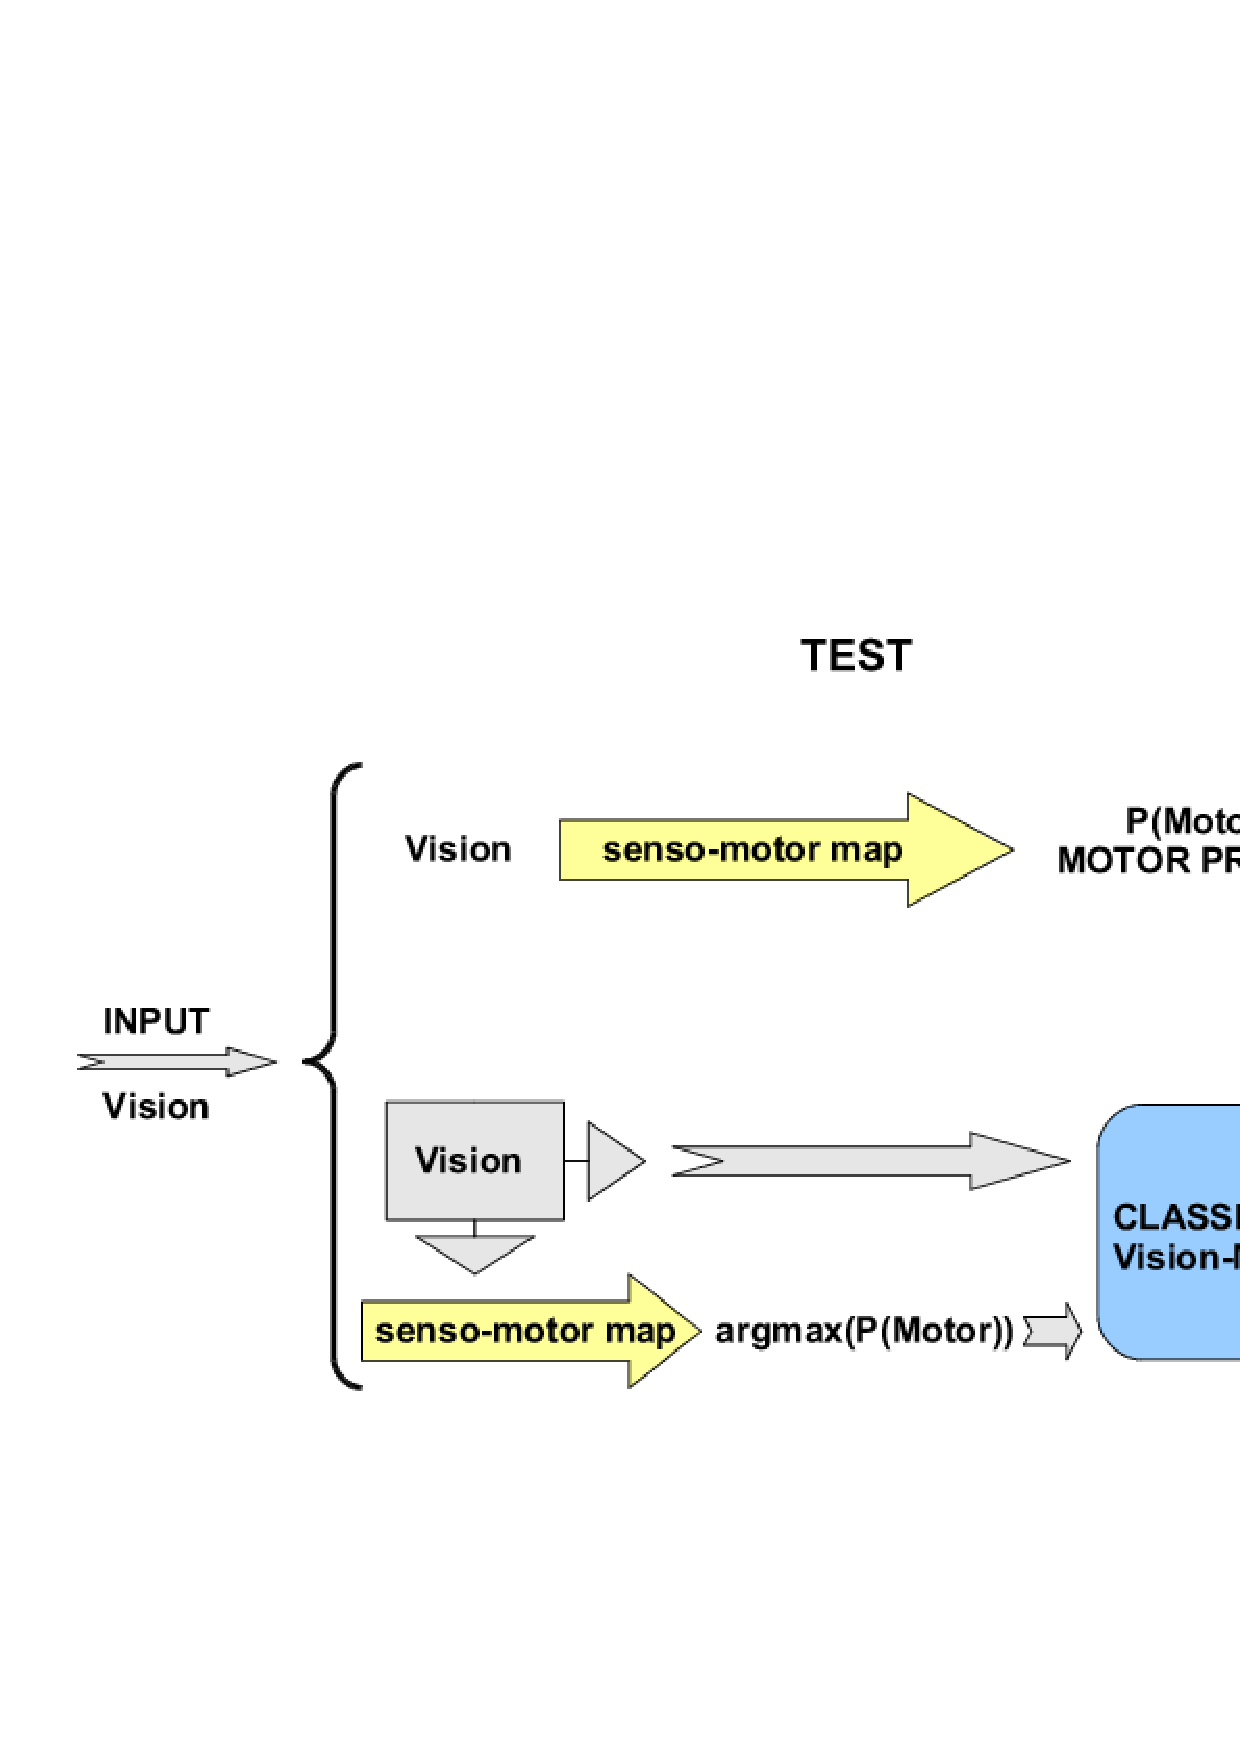
\includegraphics[width=0.7\textwidth]{images/test_fig}
%        \caption{blabla}
%        \label{fig:test-scheme}
%\end{figure}
%
%
%%\vskip -0.5cm
%
%The training phase is schematically illustrated in Figure \ref{fig:training-scheme}. During training, the system receives as input labeled visual and motor
%perceptual representation. These correspond to the seen object (Visual Perceptual Representation, VPR) and to the grasp posture of the hand
%manipulating the object (Motor Perceptual Representation, MPR). On these data, the system builds in parallel two functions: a senso-motor map
%between VPR and MPR (Figure \ref{fig:test-scheme}, top) and a classification function receiving as input both modalities, trained
%to recognize the perceived object (Figure \ref{fig:training-scheme}, bottom). Technical details on how we compute the sensor motor map and the
%multi-modal classifier are reported in section .. and ...
%
%Figure \ref{fig:test-scheme} shows the test phase with its two possible outcomes. When receiving as input a VPR of a known object, the system can
%opt for two different types of action:
%\begin{itemize}
%\item {\em Activation of the sensor-motor map}. This produces as an output an estimate of the most probable motor grasps associated 
%to that object, with the corresponding 
%MPRs for the grasp postures. We call this estimates {\em motor priming}, as they would correspond in an embodied agent to the pre-activation of the possible 
%grasps. A detailed description of how we obtain the motor priming is given in section .....
%
%\item {Object classification}. Note that, having learned the object on two modalities, the classifier needs as input a VPR and its corresponding MPR. We derive the
%{\em not perceived} MPR using the senso-motor map (Figure \ref{fig:test-scheme}, bottom). The obtained motor priming is then given as input to the classifier with the VPR. We stress again that the clasifier recognizes the object on the basis of its visual appearance and of how it can be grasped. Experiments
%reported in section ... shows clearly that this leads to a significant increase in performance compared to using only visual information.
%
%\end{itemize}
%












%\section{A theoretical framework for multi-modal learning}
%\label{sec::framework}
%
%As outlined in the Introduction, we assume that there exists a mapping between (sets of) patterns belonging to different modalities --- here we focus upon the relations which exist between a passive and an active modality. In the aforementioned example dealing with objects (as seen) and grasping them, something like what is shown in Figure \ref{fig::implementation} is sought for.
%
%\begin{figure}[h!]
%	\centering
%	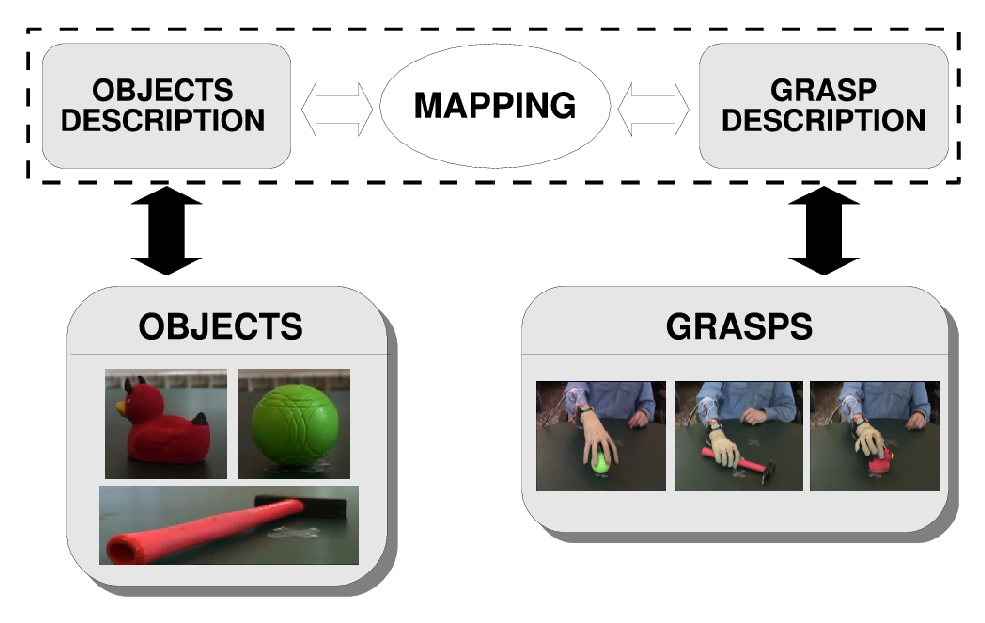
\includegraphics[width=0.7\textwidth]{images/schema_implementazione}
%	\caption{An instance of the framework we propose: estimating a
%     mapping between appropriate visual descriptions of objects and
%     classes of grasp actions. For the time being, we assume that such
%     relation is a one-to-one mapping.}
%	\label{fig::implementation}
%\end{figure}
%%\vskip -0.5cm
%
%In general, active modalities are not available to a biological system during the prediction phase, but only during the training phase. A paradigmatic example is that of a human infant learning how to grasp an object: by repeatedly trying to apply, e.g., a cylindric grasp to a bottle, he will learn not only to do it more and more efficiently, but also that a bottle is better be grasped cylindrically when moving it or bringing it close to the mouth. Later on, the sight of a bottle will remind the young human what one of the correct grasps is for that particular object. 
%A \emph{perception-to-action map} (PAM) is the equivalent of such training for a biological system: a model to reconstruct an active modality from a passive one. The PAM of our example is a mapping from visual features of an object to motor features of the grasping action used for that object. In general such a map is many-to-many: both a hammer and a bottle can be grasped cylindrically\footnote{the nomenclature of grasp types loosely follows that of Cutkosky \cite{cutkosky}.}), and as well a mug can be handled either cylindrically or by the handle. In this work we make the simplifying assumption that for a specific object there is just one acceptable grasping action --- the PAM is one-to-one.
%A PAM is useful in passive pattern recognition (e.g., classifying an object just by seeing it) since it augments the input space with PAM-reconstructed active patterns (e.g., classifying the same object from its sight \emph{and the associated grasp}). In this preliminary work we focus upon a simpler problem, namely that of checking whether, given the visual features of an object, the PAM-reconstructed grasp is (similar to) the one associated with that particular object. For example, we might train a PAM to reconstruct a pinch grip (hand posture) from the visual features of a pen; given then, in the prediciton phase, the visual features of another pen, will the PAM-reconstructed hand posture of a pinch grip look like a true pinch grip?
%
%% We consider $5$ grasp types, shown in Figure \ref{fig::grasps}, identified by different hand postures.
%
%% \begin{figure}
%% 	\centering
%% 	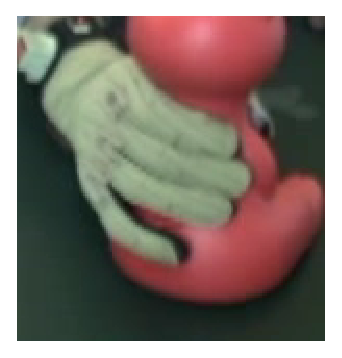
\includegraphics[width=0.19\textwidth]{images/cylinder}
%% 	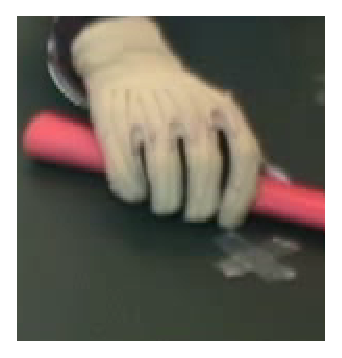
\includegraphics[width=0.19\textwidth]{images/flat}
%% 	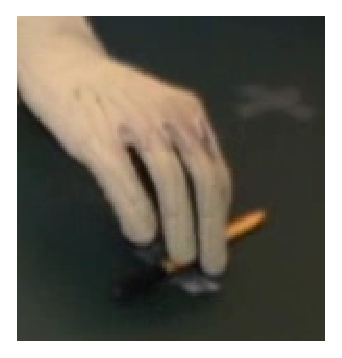
\includegraphics[width=0.19\textwidth]{images/pinch}
%% 	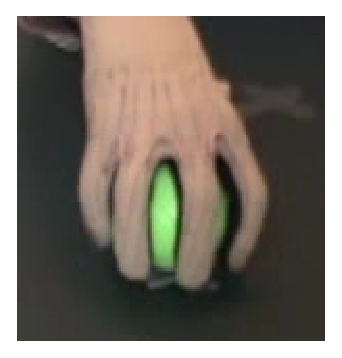
\includegraphics[width=0.19\textwidth]{images/spherical}
%% 	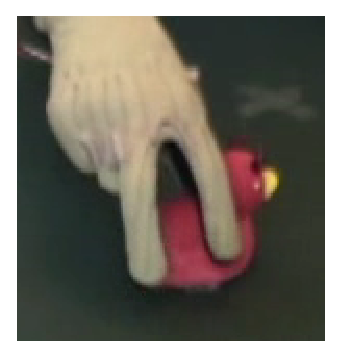
\includegraphics[width=0.19\textwidth]{images/tripodal}
%% 	\caption{The grasp types considered in this work: \emph{(left to right)}
%% 	   cylindric power grasp, flat grasp, pinch grip, spherical and
%% 	   tripodal grip.}
%% 	\label{fig::grasps}
%% \end{figure}
%
%In particular, what is needed is: $(i)$ a \emph{vision unit} to extract visual features from an image or a series of images, and $(ii)$ a \emph{regression unit}, which will build the PAM.
%%Notice that, given our assumption that this PAM is one-to-one, a simple regression method can be used to build it, i.e., we don't have to resort to probabilistic methods such as, e.g., mixture density networks, as it has been done in literature \cite{richmond}.
%
%%Among the various issues and possible applications taking shape from the general schema described so far, the problem we are interested to face can be stated as follows: supposing that it exists a relation between objects and actions, are we able to model it? Our idea is to exploit such relation to obtain joint information about object and action, that is predicting one of them given the other.\\
%%\begin{figure}
%%	\centering
%%	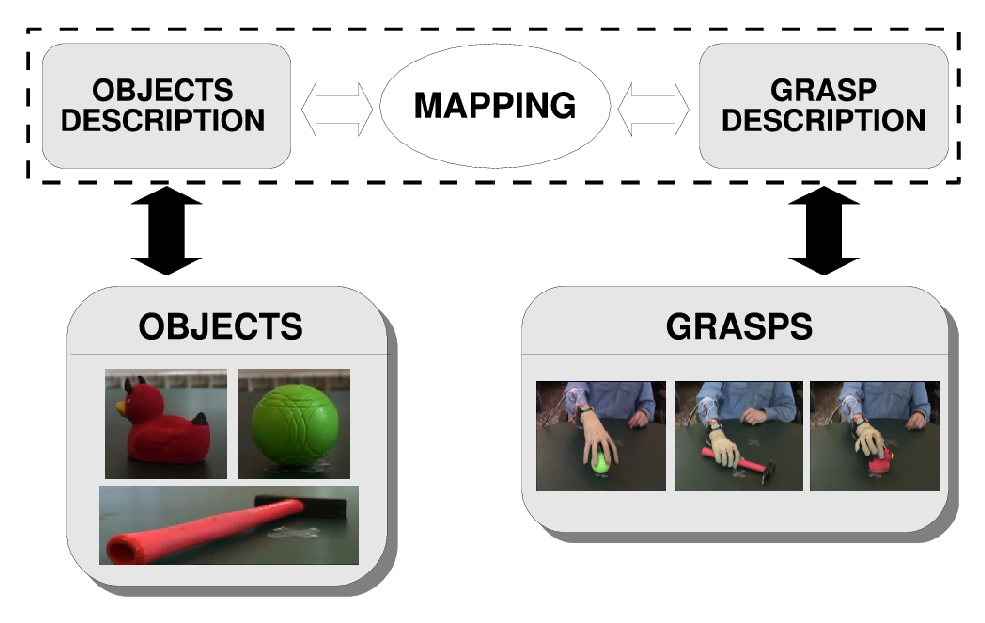
\includegraphics[width=0.7\textwidth]{images/schema_implementazione}
%%	\caption{The implementation that we consider relies on estimating a mapping between appropriate descriptions of objects and classes of grasp actions. We assume that such relation is univocally determined by knowing the object.}
%%	\label{fig::implementation}
%%\end{figure}
%%To validate this approach, we implemented a particular instance of the general schema, as shown in Fig.\ref{fig::implementation}, considering grasping actions. From the very general viewpoint we may want to consider classes of objects against classes on grasping actions. However, since our purpose here is to test the pertinence of this procedure, we start instead from the simpler hypothesis that for a specific object there is just one acceptable (class of) grasping action: in other words, we assume that the relation we are looking for can be thought of as a mono-directional mapping.\\
%%\begin{figure}
%%	\centering
%%	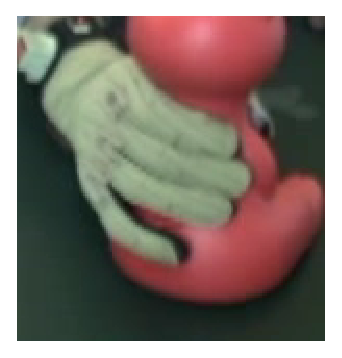
\includegraphics[width=0.19\textwidth]{images/cylinder}
%%	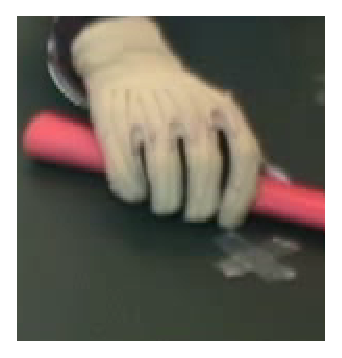
\includegraphics[width=0.19\textwidth]{images/flat}
%%	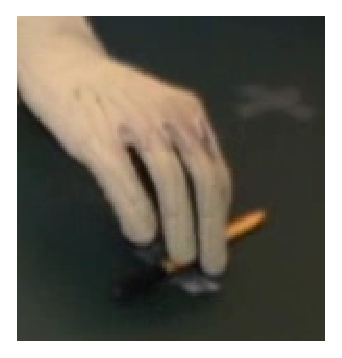
\includegraphics[width=0.19\textwidth]{images/pinch}
%%	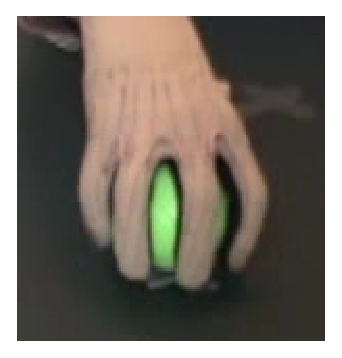
\includegraphics[width=0.19\textwidth]{images/spherical}
%%	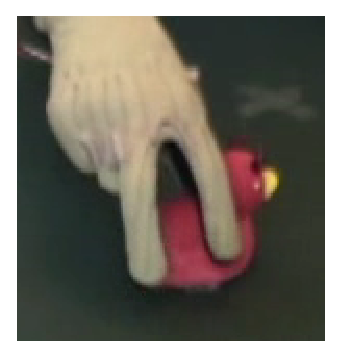
\includegraphics[width=0.19\textwidth]{images/tripodal}
%%	\caption{The different grasping types that we consider: from left to rigth, {\it cylinder power}, {\it flat}, {\it pinch}, {\it spherical} and {\it tripodal} grasp.}
%%	\label{fig::grasps}
%%\end{figure}
%%We consider 5 grasp classes, as shown in Fig. \ref{fig::grasps}, ideantified by different fingers poses.
%%To summarize, the framework we have in mind should include components able to:
%%\begin{itemize}
%%	\item model and recognize an object
%%	\item extract dynamic (visual and sensorial) information related to the action
%%	\item estimate a regression model to obtain information on dynamic actions starting from knowledge about objects appearance.
%%\end{itemize}
%%This implementation leads us to obtain a system capable of [1] modelling the relation between objects and actions in terms of mapping between appropriate descriptions to handle the multimodality, and [2] predicting the suitable grasping action for a new instance of some known object in the test phase, where motion information are not available. The latter requirement can be thought of as the capability of estimating a {\it virtual grasp}.\\
%%The system accepts in input a video signal showing object and dynamic of the action, so a natural choice lies in exploiting low-level measurements extracted from images to capture their appearance. Actions can be further described by means of sensors placed on hand and fingers, allowing to capture peculiarities typical of each grasping.\\
%%In the remainder of the paper we will introduce the strategy adopted to implement the system modules and present the preliminary results giving evidence of the pertinence of the proposed approach to solve the problem of interest.
